% Begin the document and set up the style of the document
\documentclass[a4paper,11pt]{article}

% Install the required packages for the document 
\usepackage{enumitem}
\usepackage{amsmath}
\usepackage{amssymb}
\usepackage{verbatim}
\usepackage{mathtools}
\usepackage{tikz}
\usepackage{nicefrac}
\usepackage{bm}
\usepackage{xlop}

\newcommand{\norm}[1]{\left\lVert#1\right\rVert}


% Page and style settings
%\parskip=8pt
\parindent=0pt
% Right margin
\textwidth=6.25in
% Left margin
\oddsidemargin=0pt
\evensidemargin=0pt
% Bottom margin
\textheight=10in
% Top margin
\topmargin=-0.75in
\baselineskip=11pt
% end of page and other style settings

\renewcommand{\familydefault}{\sfdefault}
\usepackage{calrsfs}
\DeclareMathAlphabet{\pazocal}{OMS}{zplm}{m}{n}

\newcommand{\indep}{\mathrel{\text{\scalebox{1.07}{$\perp\mkern-10mu\perp$}}}}
\newcommand{\p}{\mathbb{P}}
\newcommand{\e}{\mathbb{E}}
\newcommand{\ds}{\displaystyle}
\newcommand{\code}{\texttt}
\newcommand{\HRule}{\rule{\linewidth}{0.5mm}} % Defines a new command for the horizontal lines, change thickness here

\newenvironment{nscentre}
 {\parskip=0pt\par\nopagebreak\centering}
 {\par\noindent\ignorespacesafterend}


\usepackage{fullpage}

\usepackage{titlesec} % Used to customize the \section command
\titleformat{\section}{\bf}{}{0em}{}[\titlerule] % Text formatting of sections
\titlespacing*{\section}{0pt}{3pt}{3pt} % Spacing around sections

\begin{document}
\setlength{\abovedisplayskip}{8pt}{%
\setlength{\belowdisplayskip}{8pt}{%


\text{LSA}
\hfill
\text{University of Michigan}

\begin{nscentre}
	\textbf{MATH562: Continuous Optimisation}\\
	\textbf{Homework 2}\\
\end{nscentre}

\text{Name: Keegan Gyoery}
\hfill
\text{UM-ID: 31799451}

\pagenumbering{arabic}
	\begin{enumerate}[leftmargin=*]
		\item \textbf{A:} min $\ds{f(\mathbf{x}) = x_1 + x_2 - \ln{x_1} - \ln{x_2}}$
			\begin{enumerate}[label=\alph*)]

				\item The first order necessary condition a point must satisfy is $\ds{\nabla f(\mathbf{x}) = \mathbf{0}}$. Considering the gradient of $\ds{f(\mathbf{x})}$,
					\begin{align*}
						\nabla f(\mathbf{x}) & = \left(1-\frac{1}{x_1}, \: 1-\frac{1}{x_2}\right). 
					\end{align*}
					Thus, the necessary condition for a point to be a minimum is $\ds{\left(1-\frac{1}{x_1}, \: 1-\frac{1}{x_2}\right) = (0,0)}$.

			\item Considering the conditions from above, 
				\begin{align*}
					1 - \frac{1}{x_1} & = 0 \\
					\therefore x_1 & = 1, \\
					1 - \frac{1}{x_2} & = 0 \\
					\therefore x_2 & = 1.
				\end{align*}
				Thus, the point $\ds{\hat{\mathbf{x}} = (1,1)}$ satisfies the necessary condition for a local minimum.
			\item Considering the Hessian of $\ds{f(\mathbf{x})}$, and $\ds{\mathbf{h} = (h_1,h_2) \neq \mathbf{0}}$,
				\begin{align*}
					Hf(\mathbf{x}) & =
					\begin{bmatrix}
						\frac{1}{x_1^2} & 0 \\
						0 & \frac{1}{x_2^2} \\
					\end{bmatrix}, \\
					\mathbf{h}^T Hf(\mathbf{x})\mathbf{h} & = \mathbf{h}^T
					\begin{bmatrix}
						\frac{1}{x_1^2} & 0 \\
						0 & \frac{1}{x_2^2} \\
					\end{bmatrix}\mathbf{h} \\
					& =\frac{h_1^2}{x_1^2} + \frac{h_2^2}{x_2^2} \\
					& > 0 \: \forall \mathbf{h},\mathbf{x}.
				\end{align*}
				Thus $\ds{Hf(\mathbf{x})}$ is P.S.D and P.D, and so too is $\ds{Hf(\hat{\mathbf{x}})}$. Clearly, $\ds{\hat{\mathbf{x}}}$ satisfies the second order necessary condition and the two second order sufficient conditions, and so $\ds{\hat{\mathbf{x}}}$ is a local minimum.
					

			\end{enumerate}
			\textbf{B:} min $\ds{f(\mathbf{x}) = 2\ln(x_1 + x_2+1) - \ln{x_1} - 1.5\ln{x_2}}$
			\begin{enumerate}[label=\alph*)]

				\item The first order necessary condition a point must satisfy is $\ds{\nabla f(\mathbf{x}) = \mathbf{0}}$. Considering the gradient of $\ds{f(\mathbf{x})}$,
					\begin{align*}
						\nabla f(\mathbf{x}) & = \left(\frac{2}{x_1+x_2+1} - \frac{1}{x_1}, \: \frac{2}{x_1+x_2+1}-\frac{1.5}{x_2}\right). 
					\end{align*}
					Thus, the necessary condition for a point to be a minimum is \\ $\ds{\left(\frac{2}{x_1+x_2+1} - \frac{1}{x_1}, \: \frac{2}{x_1+x_2+1}-\frac{1.5}{x_2}\right) = (0,0)}$.

			\item Considering the conditions from above, 
				\begin{align*}
					\frac{2}{x_1+x_2+1} - \frac{1}{x_1} & = 0 \\
					2x_1 & = x_1 + x_2 + 1 \\
					\therefore x_2 & = x_1 - 1 \dots (A),\\
					\frac{2}{x_1+x_2+1}-\frac{1.5}{x_2} & = 0 \\
					2x_2 & = 1.5x_1 + 1.5x_2 + 1.5 \\
					\therefore x_2 & = 3x_1 + 3 \dots(B).
				\end{align*}
				Combining equations $\ds{(A)}$ and $\ds{(B)}$, 
				\begin{align*}
					x_1 - 1 & = 3x_1 + 3 \\
					\therefore x_1 & = -2 \\
					\therefore x_2 & = -3
				\end{align*}
				Thus, the point $\ds{\hat{\mathbf{x}} = (-2,-3)}$ satisfies the necessary condition for a local minimum.
			\item Considering the Hessian of $\ds{f(\mathbf{x})}$, and $\ds{\mathbf{h} = (h_1,h_2) \neq \mathbf{0}}$,
				\begin{align*}
					Hf(\mathbf{x}) & =
					\begin{bmatrix}
						\frac{-2}{(x_1+x_2+1)^2} + \frac{1}{x_1^2} & \frac{-2}{(x_1+x_2+1)^2} \\
						\frac{-2}{(x_1+x_2+1)^2} & \frac{-2}{(x_1+x_2+1)^2} + \frac{1}{x_1^2} \\
					\end{bmatrix}, \\
					\therefore Hf(-2,-3) & = 
					\begin{bmatrix}
						\frac{1}{8} & -\frac{1}{8} \\
						-\frac{1}{8} & \frac{1}{24} \\
					\end{bmatrix}, \\
					\mathbf{h}^T Hf(-2,-3)\mathbf{h} & = \mathbf{h}^T
					\begin{bmatrix}
						\frac{1}{8} & -\frac{1}{8} \\
						-\frac{1}{8} & \frac{1}{24} \\
					\end{bmatrix}\mathbf{h} \\
					& =\frac{h_1^2}{8} - \frac{h_1h_2}{4} + \frac{h_2^2}{24} \\
				\end{align*}
				Consider $\ds{\mathbf{h} = (1,1)}$, 
				\begin{align*}
					\mathbf{h}^T Hf(-2,-3)\mathbf{h} & = (1,1)^T Hf(-2,-3) (1,1)\\
													 & = \frac{1}{8} - \frac{1}{4} + \frac{1}{24} \\
													 & = -\frac{1}{12}\\
													 & < 0.
				\end{align*}
				Thus $\ds{Hf(\hat{\mathbf{x}})}$ is not P.D or P.S.D, so $\ds{\hat{\mathbf{x}}}$ fails the second order necessary condition, and thus cannot be a local minimum. 

			\end{enumerate}
			\textbf{C:} min $\ds{f(\mathbf{x}) = x_1x_2 - \ln{x_1} - \ln{x_2}}$
			\begin{enumerate}[label=\alph*)]

				\item The first order necessary condition a point must satisfy is $\ds{\nabla f(\mathbf{x}) = \mathbf{0}}$. Considering the gradient of $\ds{f(\mathbf{x})}$,
					\begin{align*}
						\nabla f(\mathbf{x}) & = \left(x_2-\frac{1}{x_1}, \: x_1-\frac{1}{x_2}\right). 
					\end{align*}
					Thus, the necessary condition for a point to be a minimum is $\ds{\left(x_2-\frac{1}{x_1}, \: x_1-\frac{1}{x_2}\right) = (0,0)}$.

			\item Considering the conditions from above, 
				\begin{align*}
					x_2 - \frac{1}{x_1} & = 0 \\
					\therefore x_1x_2 & = 1, \\
					x_1 - \frac{1}{x_2} & = 0 \\
					\therefore x_1x_2 & = 1.
				\end{align*}
				Thus, the point $\ds{\hat{\mathbf{x}} = \left(t,\frac{1}{t}\right)}$ satisfies the necessary condition for a local minimum.
			\item Considering the Hessian of $\ds{f(\mathbf{x})}$, and $\ds{\mathbf{h} = (h_1,h_2) \neq \mathbf{0}}$,
				\begin{align*}
					Hf(\mathbf{x}) & =
					\begin{bmatrix}
						\frac{1}{x_1^2} & 1 \\
						1 & \frac{1}{x_2^2} \\
					\end{bmatrix}, \\
					\therefore \mathbf{h}^T Hf(\mathbf{x})\mathbf{h} & = \mathbf{h}^T
					\begin{bmatrix}
						\frac{1}{x_1^2} & 1 \\
						1 & \frac{1}{x_2^2} \\
					\end{bmatrix} \mathbf{h} \\
					& =\frac{h_1^2}{x_1^2} + 2h_1h_2 + \frac{h_2^2}{x_2^2} \\
					& = \left(\frac{h_1}{x_1} + \frac{h_2}{x_2}\right)^2 \\
					& > 0 \: \forall \mathbf{h},\mathbf{x}.
				\end{align*}
				Thus $\ds{Hf(\mathbf{x})}$ is P.S.D and P.D, and so too is $\ds{Hf\left(t,\frac{1}{t}\right)}$. Clearly, $\ds{\hat{\mathbf{x}}}$ satisfies the second order necessary condition and the two second order sufficient conditions, and so $\ds{\hat{\mathbf{x}}}$ is a local minimum.
					

			\end{enumerate}

		\item Consider the problem
			\begin{align*}
				\min f(\mathbf{x}) & = 5(x_1^2 - x_2)^2 + x_1^2 + (x_2-5)^2
			\end{align*}
			\begin{enumerate}[label=\alph*)]
				\item The gradient and Hessian for the function $\ds{f(\mathbf{x})}$ are
					\begin{align*}
						\nabla f(\mathbf{x}) & = \left(20x_1^3-20x_1x_2+2x_1, -10x_1^2+12x_2-10\right), \\
						Hf(\mathbf{x}) & = 
						\begin{bmatrix}
							60x_1^2-20x_2+2 & -20x_1 \\
							-20x_1 & 12 \\
						\end{bmatrix}.
					\end{align*}
				\item Considering the neccessary and sufficient conditions for a P.S.D. matrix, we get the restrictions,
					\begin{align*}
						60x_1^2-20x_2+2 & \geq 0 \dots (1), \\
						12 & \geq 0, \text{ which is true,} \\
						12(60x_1^2-20x_2+2) - 400 x_1^2 & \geq 0 \\
						\therefore 40x_1^2 - 30x_2 + 3 & \geq 0 \dots (2).
					\end{align*}

				\item To check that $\ds{\hat{\mathbf{x}} = \left(0,\frac{5}{6}\right)}$ is a local minimum, it must first satisfy the first and second order necessary conditions. Examining the gradient at $\ds{\hat{\mathbf{x}}}$, and the restrictions above,
					\begin{align*}
						\nabla f\left(0, \frac{5}{6} \right) & = (0,0) \\
						(2) & \rightarrow -22 \ngeq 0. \\
					\end{align*}
					Thus, $\ds{Hf\left(0, \frac{5}{6}\right)}$ is not P.S.D., and so $\ds{\hat{\mathbf{x}}}$ cannot be a local minimum.

			\end{enumerate}

		\item Using the MATLAB code,
			\begin{figure}[h!]
				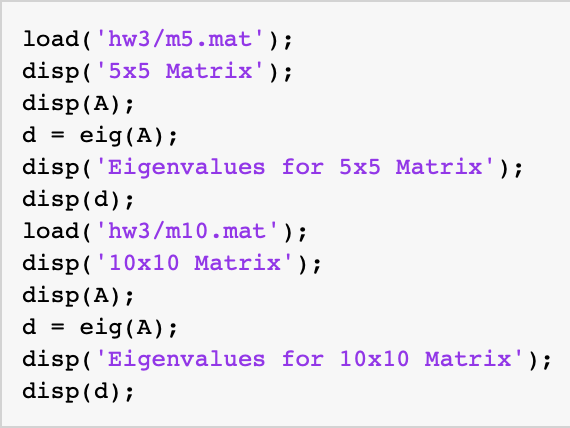
\includegraphics[width=\linewidth]{code.png}
			\end{figure}\\
			we get the output for the 5x5 matrix,
			\pagebreak
			\begin{figure}[h!]
				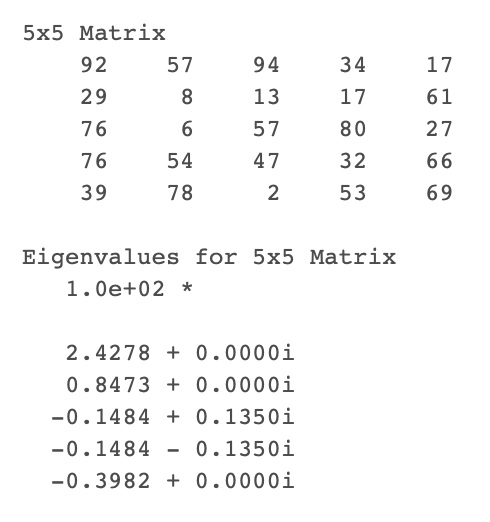
\includegraphics[width=\linewidth]{5.png}
			\end{figure}.\\
			Clearly, this matrix is not even symmetric and and thus cannot be P.D. or P.S.D.

			From the output for the 10x10 matrix,
			\pagebreak
			\begin{figure}[h!]
				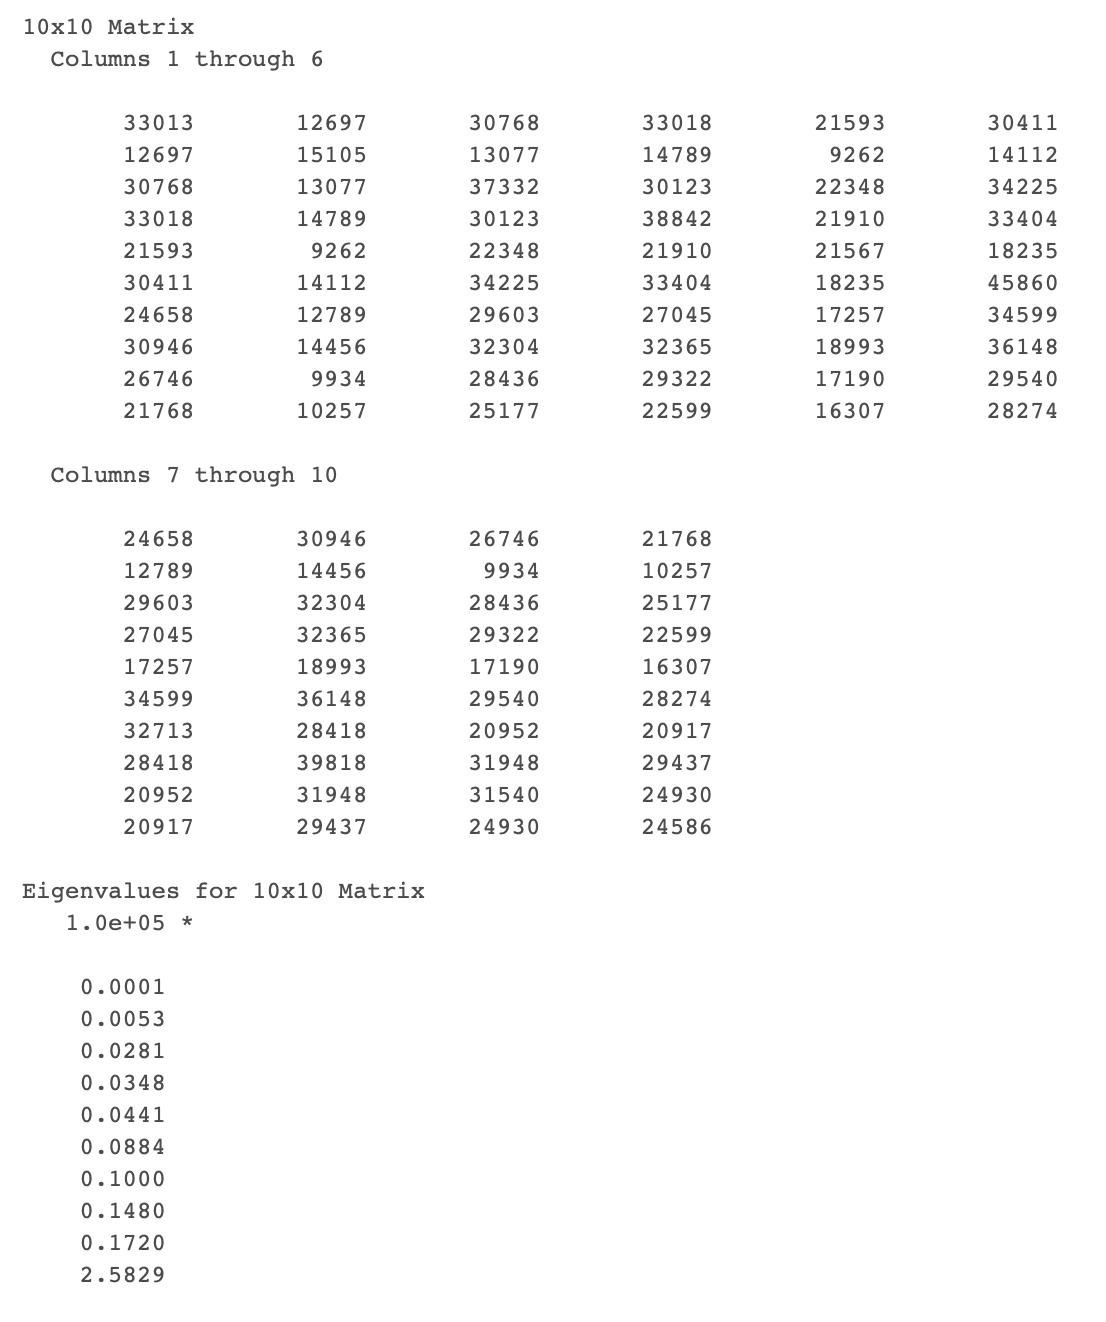
\includegraphics[width=\linewidth]{10.png}
			\end{figure}.\\
			We can clearly see that all the eigenvalues are positive, and thus, the matrix is P.D.


		\pagebreak
		\item Suppose $\ds{M}$ is P.D.
			\begin{enumerate}[label=\alph*)]
				\item If $\ds{M}$ is P.D., then $\ds{M}$ has all positive eigenvalues. Thus, no eigenvalue of $\ds{M}$ is $\ds{0}$, and hence $\ds{M}$ is invertible, and thus $\ds{M^{-1}}$ exists. By definition, $\ds{M^{-1}M = I}$, and noting M is symmetric, so taking the transpose gives,
					\begin{align*}
						\left(M^{-1}M\right)^T & = I^T \\
						M^T\left(M^{-1}\right)^T & = I \\
						M\left(M^{-1}\right)^T & = I \\
						\therefore \left(M^{-1}\right)^T & = M^{-1}.
					\end{align*}
					Thus, $\ds{M^{-1}}$ is real and symmetric. Finally, condsider the eigenvalues $\ds{\lambda_i}$ of $\ds{M}$, given by $\ds{M\mathbf{x} = \lambda \mathbf{x}}$. Manipulating for $\ds{M^{-1}}$,
					\begin{align*}
						M\mathbf{x} & = \lambda \mathbf{x} \\
						\therefore \mathbf{x} & = M^{-1} \lambda \mathbf{x} \\
											  & = \lambda M^{-1} \mathbf{x} \\
						\therefore \frac{1}{\lambda} \mathbf{x} & = M^{-1} \mathbf{x} \\
						\therefore M^{-1} \mathbf{x} & = \frac{1}{\lambda} \mathbf{x}.
					\end{align*}
					Clearly, the eigenvalues of $\ds{M^{-1}}$ are $\ds{\frac{1}{\lambda_i}}$, which are all positive. Thus, $\ds{M^{-1}}$ is P.D.
				\item Refer to the proof above, showing that the eigenvalues of $\ds{M^{-1}}$ are the inverse of the eignevalues of $\ds{M}$.
				\item Let $\ds{\mathbf{u}}$ be an eigenvector of $\ds{M}$, where $\ds{\lambda}$ is the associated eigenvalue. Thus,
					\begin{align*}
						M\mathbf{u} & = \lambda \mathbf{u} \\
						\mathbf{u} & = M^{-1} \lambda \mathbf{u} \\
						\therefore M^{-1} \mathbf{u} & = \frac{1}{\lambda} \mathbf{u}.
					\end{align*}
					Clearly, $\ds{\mathbf{u}}$ is an eigenvector of $\ds{M^{-1}}$ with eigenvalue $\ds{\frac{1}{\lambda}}$. Now let $\ds{\mathbf{u}}$ be an eigenvector of $\ds{M^{-1}}$, where $\ds{\frac{1}{\lambda}}$ is the associated eigenvalue. Thus,
					\begin{align*}
						M^{-1}\mathbf{u} & = \frac{1}{\lambda} \mathbf{u} \\
						\mathbf{u} & = M \frac{1}{\lambda} \mathbf{u} \\
						\therefore M \mathbf{u} & = \lambda \mathbf{u}.
					\end{align*}
					Clearly, $\ds{\mathbf{u}}$ is an eigenvector of $\ds{M}$ with eigenvalue $\ds{\lambda}$.
			\end{enumerate}

		\item Suppose that $\ds{M}$ is P.S.D. Therefore, $\ds{M}$ is real and symetric, and so can be rewritten $\ds{M = QDQ^T}$, where $\ds{Q}$ is orthonormal, and $\ds{D}$ is diagonal, with the eigenvalues of $\ds{M}$ along the diagonal. All eigenvalues of $\ds{M}$ are non-negative, and so let $\ds{N}$ be given by $\ds{QLQ^T}$, where $\ds{Q}$ is the same as above, and $\ds{L}$ is another diagonal matrix with the square root of the eigenvalues of $\ds{M}$ along the diagonal. That is, $\ds{D = \text{diag}[\lambda_1 \: \lambda_2 \: \dots \: \lambda_n]}$, and $\ds{L = \text{diag}[\sqrt{\lambda_1} \: \sqrt{\lambda_2} \: \dots \: \sqrt{\lambda_n}]}$. Noting that because $\ds{Q}$ is orthonormal, $\ds{Q^T = Q^{-1}}$, and so, 
			\begin{align*}
				N^2 & = NN \\
					& = \left(QLQ^T\right)\left(QLQ^T\right) \\
					& = \left(QL\right)\left(QQ^T\right)\left(LQ^T\right) \\
					& = \left(QL\right)\left(I\right)\left(LQ^T\right) \\
					& = \left(QL\right)\left(LQ^T\right) \\
					& = \left(QLLQ^T\right) \\
					& = \left(QL^2Q^T\right) \\
					& = \left(QDQ^T\right) \\
				\therefore N^2 & = M. 
			\end{align*}
			As $\ds{N = QLQ^T}$, the eigenvalues of $\ds{N}$ are all non-negative, and as $\ds{N}$ is written in the above form, where $\ds{L}$ is diagonal and $\ds{Q}$ is orthonormal, then $\ds{N}$ is also P.S.D. Thus, there exists an $\ds{N}$ P.S.D. such that $\ds{N^2 = M}$.


	\end{enumerate}
\end{document}
